\chapter{Experiment Setup} \label{Chp: Setup}
%All experiments are done within the Cooja simulator. The environment we simulated is as described in \Cref{fig: Setup}.

In this chapter we describe how we set up our experiments. The related source code can be downloaded from:\\
\begin{center}
	\url{https://github.com/Salties/MyRepository}
\end{center}

\section{Overview}

\Cref{Fig: Experiment Setup} illustrates an overview of our experiment setup. We explain the components of our experiments in \Cref{Fig: Experiment Setup}.

\begin{figure*}[h!]
	\center
	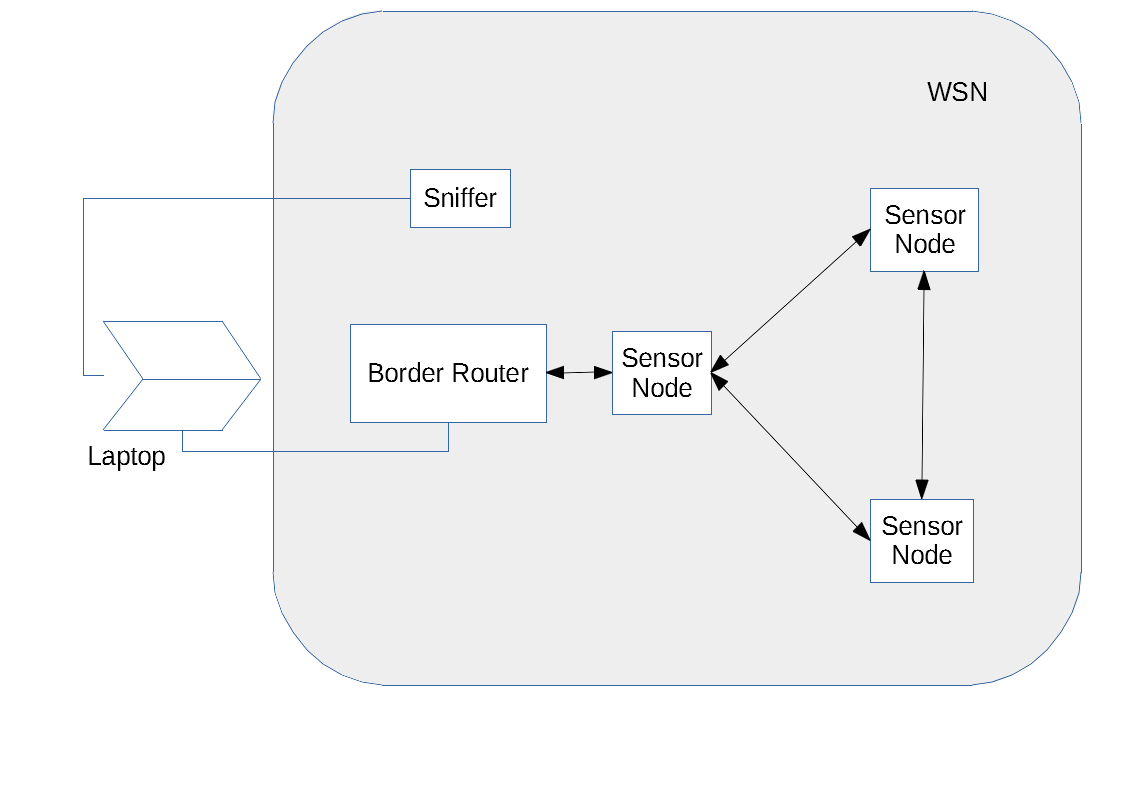
\includegraphics[width=0.75\textwidth,]{fig/setup.png}
	\caption{Experiment Setup} \label{Fig: Experiment Setup}
\end{figure*}

\begin{description}[style=nextline]
	\item[Sensor Network]
	The greyed area on the right inside the rectangle of \Cref{Fig: Experiment Setup} represents a WSN application.  The topology is dynamic and can change due to the application.  We make no further assumptions about the exact application at this point for generality.
	
	\item[Sensor Node]
	Each Sensor Node is a device with support of the protocol suite described in \Cref{Tbl: Summary of WSN Building Blocks}. All Sensor Nodes are connected to the same 6LoWPAN network. We do not impose the use of CoAP in our setup; instead, we assume applications may directly use the interface of UDP( or DTLS). More details are  are given in the later sections.
	
	\item[Border Router]
	Border Router is a special instance of Sensor Node. In addition to RF, Border Routers are additionally connected to other devices via different connections. In the experiments of this project, Border Routers are connected to a laptop through a USB connection. Border Router bridges two network. In the scenario of \Cref{Fig: Experiment Setup}, the Border Router is used to transmit IPv6 packets sent from the laptop. From a perspective of other Sensor Nodes in the WSN, a Border Router appears no different to the others. In many real world applications, the Border Router is connected to a management machine and serves as the DODAG root but this is not necessary in this experiment.
	
	\item[Sniffer]
	Sniffer is another special instance of Sensor Node. The Sniffer passively captures all frames it receives and does not transmit anything at all; thus it is transparent to other Sensor Nodes in the network. In our setup as of \Cref{Fig: Experiment Setup}, the Sniffer pipes any frames it captured to the Laptop. From a practical perspective, the hardware device of a Sniffer has a limited effective radius and thus would not be able to capture all frames in WSNs of wide deployment; however this can be easily overcame by deploying multiple synchronised Sniffers to cover a wide area. In our experiments, we assume every frame in the network is captured by the Sniffer.
	
	\item[Laptop]
	The Laptop in our experiment represents an adversary with unequally supreme resources comparing to the Sensor Nodes in terms of energy, memory and computational power. In our setup of \Cref{Fig: Experiment Setup}, the Laptop, which also represents the adversary, has access to all traffic captured by the Sniffer and is allowed to interact with other Sensor Nodes through the Border Router if authentication is not required to join the network.
\end{description}

\section{Operating System}

We use Contiki\cite{Contiki} to build our experiments.  Our source code are tested  with the release version of Contiki 3.0 which is available at:

\begin{center}
	\url{https://github.com/contiki-os/contiki/releases/tag/3.0}.
\end{center}

\subsection{Brief Introduction to Contiki:}

The official instruction for using Contiki is available at:
\begin{center}
	\url{http://www.contiki-os.org/start.html}
\end{center}

Contiki is an open source embedded system crafted for IoT devices. It has a good support on many recent hardware and it is optimised for code size. Comparing to Operating Systems for PCs, Contiki does not provide a User Interface, UI. Instead, the embedded system provides a framework for developers to use C language to write (mostly) hardware portable codes, as well as a set of APIs including clock library, simple process management and network interfaces,etc.

To use Contiki, there are basically three steps:

\begin{enumerate}
	\item Write the application code in C. There are plenty of code in the Contiki example folder that can be used as frameworks.
	\item Compile the source code according to the target device through \textit{make} command. Note that the root of Contiki source code must be correctly specified in the \textit{makefile}.
	\item Upload (also called ``burn'') the binary code to your device. 
\end{enumerate}

The application code is automatically executed whenever the device is powered on.

\section{Devices}

Three models of device are adopted in this project:

\begin{itemize}
	\item \textbf{TelosB}\cite{TelosB}, as known as Sky mote. This is a popular model for WSNs featuring low cost. As a trade off, TelosB has only very constrained performance in terms of bandwidth, available code size and processing power.
	
	\item \textbf{CC2538}\cite{CC2538}. This is a relatively powerful model with an ARM-Cortex M3 processor. To our knowledge, this is one of the becoming dominant device used in WSN applications.
	
	\item \textbf{Wismote}\cite{Wismote}. This model is used as a performance upgraded version of TelosB in this project. In this project, Wismote \textbf{IS ONLY USED IN SIMULATIONS}. 
\end{itemize}

All these nodes are 802.15.4\cite{802154} compatible and does not have any sensor attached by default. We omit further hardware details as it is beyond the scope of this project. 

\subsection{Cooja Simulator}

The Contiki source code includes the Cooja simulator under its tools folder. The official instruction of using the Cooja simulator is available at 

\begin{center}
	\url{http://www.contiki-os.org/start.html}
\end{center}

Cooja provides simulation for a whole WSN application. It generates simulation data for serial output, LED status and radio traffic. An example of Cooja execution is shown in \Cref{Fig: An Example of Cooja Execution}.

\begin{figure*}[h!]
	\center
	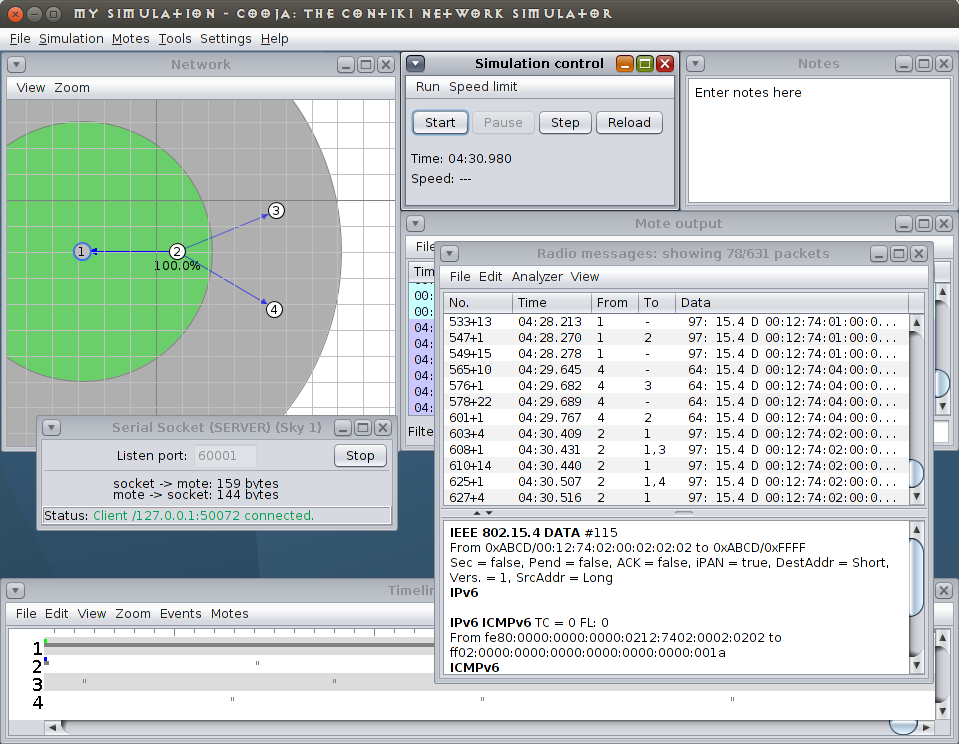
\includegraphics[width=0.8\textwidth]{fig/cooja_example.png}
	\caption{An Example of Cooja Execution}
	\label{Fig: An Example of Cooja Execution}
\end{figure*}

\Cref{Fig: An Example of Cooja Execution} shows a simulation simulating the exact same WSN topology as described in \Cref{Fig: Experiment Setup}, with \textcircled{1} being the Border Router. 

In this project, we are mostly interested in the radio traffic. The traffic is captured by the ``Radio messages'' plugin which corresponds to the Sniffer in \Cref{Fig: Experiment Setup}. The corresponding pcap file is written by Cooja alongside the simulation under ``cooja/build/'' folder, which can later be opened by Wireshark\cite{Wireshark} for analysis, as shown in \Cref{Fig: A Wireshark Example}.

\begin{figure*}[h!]
	\center
	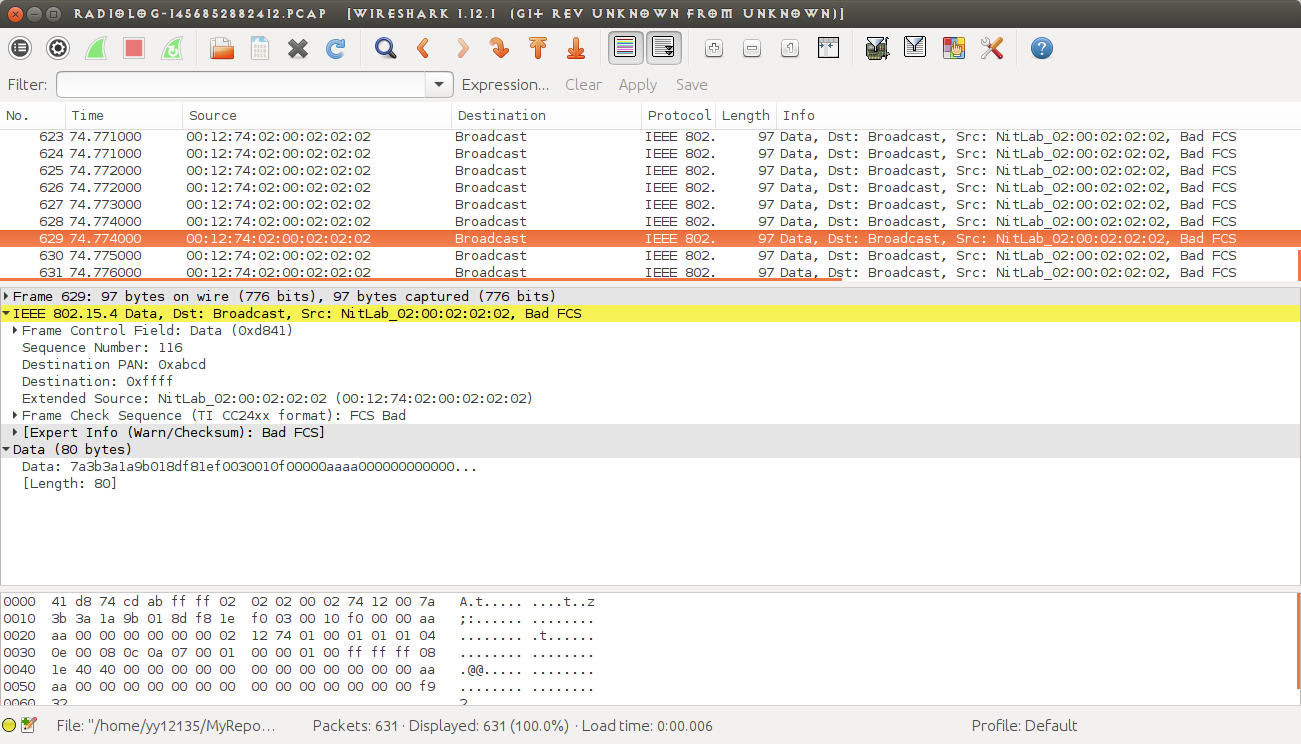
\includegraphics[width=0.8\textwidth]{fig/wireshark_example.png}
	\caption{A Wireshark Example}
	\label{Fig: A Wireshark Example}
\end{figure*}

As of the time of writing this report, Cooja in Contiki release 3.0 supports simulation for TelosB and Wismote. CC2538 is not yet supported in the current version.

\section{Security Measures}

In this report we use two security measures those are implemented on Contiki, namely noncoresec and DTLS.

\subsection{noncoresec}

\textit{noncoresec}\cite{noncoresec}\cite{LLSEC} is a simplified 802.15.4 Security implementation on Contiki. \textit{noncoresec} uses a hard coded network shared key that is defined by the ``NONCORESEC\_CONF\_KEY'' macro in ``project-conf.h'' file; thus it cannot be updated during runtime. 

When \textit{noncoresec} is enabled, we always assume it uses the highest Security Level (7), i.e. all frames are encrypted and authenticated in AES-128-CCM* mode with 16 bytes MAC, as described in \Cref{Subsec: 802154 Sec}. With this Security Level, all Sensor Nodes in the WSN must have the same key hard coded into the Contiki kernel. Sensor Nodes without the key cannot send or receive any frame.

In scenarios where the WSN is protected by \textit{noncoresec}, we always assume the adversary has no knowledge of the key. This effectively indicates that the adversary is unable to join the network at all since he cannot receive or send any frames.

Our code using \textit{noncoresec} are successfully tested on all our devices. However, even though CC2538 has an AES coprocessor built in, the current version of Contiki code does not utilise this feature at all; instead, it uses a textbook software AES implementation as on TelosB and Wismote. Also notice that the source code of \textit{noncoresec} is only included for TelosB platform by default. When using with other platforms, the developer needs to manually add its source code into the corresponding building system.

\subsection{DTLS}

\section{Applications}

\section{Summary}

%A table for available combinations

%\begin{itemize}
%\item{\bf Adversary} is a malicious party that tries to illegally reveal information from the encrypted traffic.
%\item{\bf Border Router}, or BR, is a device that connects adversary to the sensor network. \textbf{BR is not allowed when LLSEC is enabled} as the adversary does not have the key and hence cannot connect into the network. We will discuss more about LLSEC in \Cref{Chp: LLSEC}.
%\item{\bf Sniffer} passively captures all traffic in the network. 
%\item{\bf Target} and {\bf Nodes} are sensors deployed in the sensor network. They communicates to each other through encrypted channels.
%\item{\bf Sensor Network} discussed in this paper is a 6LowPAN network based on Contiki OS.
%\end{itemize}

%Realistically speaking, this scenario could happen say an adversary sitting near a smart house with a laptop attached to a SoC\footnote{System on Chip} device, or your malicious neighbour walks into your smart house with her smart phone.
%
%\section{Adversary Power}
%The powers assumed in the experiments are considered to be practical in real life.
%
%When LLSEC is enabled, all traffic, including RPL\footnote{Routing Procol for Low-power and Lossy Networks} messages, are encrypted; therefore no external nodes can connect to the network as an external node cannot send any valid RPL messages to join the network. The adversary only passively sniffs all traffic.
%
%With LLSEC disabled, the adversary can therefore join the sensor network through a BR and hence is also capable to send messages to the target(s). However, she will not be able to inject any message into an encrypted channel such as a DTLS channel.
%
%\section{Types of Packets}
%We simply categorise the packets into two types:
%\begin{itemize}
%\item {\bf Network Management Packets}: These are the packets generated by the protocols to  maintain the functionality of network, such as MAC ACKs, RPL messages or ICMP messages.
%\item {\bf Data Packets}: These are those packets generated by applications running on sensor nodes., such as a CoAP packet.
%\end{itemize}
%
%This is only a subjective rough categorisation and may not be precise. For example an TCP data packet may set its ACK flag, or DTLS handshake packets could ambiguously fall into both categories. However, we ignore this ambiguity as it is not our focus.